% $Header: /cvsroot/latex-beamer/latex-beamer/solutions/conference-talks/conference-ornate-20min.en.tex,v 1.6 2004/10/07 20:53:08 tantau Exp $

\documentclass{beamer}

% This file is a solution template for:

% - Talk at a conference/colloquium.
% - Talk length is about 20min.
% - Style is ornate.



% Copyright 2004 by Till Tantau <tantau@users.sourceforge.net>.
%
% In principle, this file can be redistributed and/or modified under
% the terms of the GNU Public License, version 2.
%
% However, this file is supposed to be a template to be modified
% for your own needs. For this reason, if you use this file as a
% template and not specifically distribute it as part of a another
% package/program, I grant the extra permission to freely copy and
% modify this file as you see fit and even to delete this copyright
% notice.


\mode<presentation>
{
%  \usetheme{Warsaw}
%  \usetheme{Boadilla}
%  \usetheme{Goettingen}
%  \usetheme{Hannover}
%  \usetheme{Madrid}
%  \usetheme{Marburg}
%  \usetheme{Montpellier}
%  \usetheme{Pittsburgh}
  \usetheme{Hawke}
  % or ...

  \setbeamercovered{transparent}
  % or whatever (possibly just delete it)
}


\usepackage[english]{babel}
% or whatever

\usepackage[latin1]{inputenc}
% or whatever

\usepackage{times}
\usepackage[T1]{fontenc}
% Or whatever. Note that the encoding and the font should match. If T1
% does not look nice, try deleting the line with the fontenc.

\usepackage{multimedia}


%%%%%%
% My Commands
%%%%%%

\usepackage{SULectureMathsSlides}
\newcommand{\ml}{{\sc matlab}}
\newcommand{\bfm}[1]{{\boldsymbol{#1}}}
%\newcommand{\bx}{\bfm{x}}

%%%%

\title[Lecture 10] % (optional, use only with long paper titles)
{Lecture 10 - Roots of Nonlinear Systems}

% \subtitle
% {Include Only If Paper Has a Subtitle}

\author[I. Hawke] % (optional, use only with lots of authors)
{I.~Hawke}
% - Give the names in the same order as the appear in the paper.
% - Use the \inst{?} command only if the authors have different
%   affiliation.

\institute[University of Southampton] % (optional, but mostly needed)
{
%  \inst{1}%
  School of Mathematics, \\
  University of Southampton, UK
}
% - Use the \inst command only if there are several affiliations.
% - Keep it simple, no one is interested in your street address.

\date[Semester 1] % (optional, should be abbreviation of conference name)
{MATH3018/6141, Semester 1}
% - Either use conference name or its abbreviation.
% - Not really informative to the audience, more for people (including
%   yourself) who are reading the slides online

\subject{Numerical methods}
% This is only inserted into the PDF information catalog. Can be left
% out.



% If you have a file called "university-logo-filename.xxx", where xxx
% is a graphic format that can be processed by latex or pdflatex,
% resp., then you can add a logo as follows:

\pgfdeclareimage[height=0.5cm]{university-logo}{mathematics_7469}
\logo{\pgfuseimage{university-logo}}



% Delete this, if you do not want the table of contents to pop up at
% the beginning of each subsection:
%  \AtBeginSubsection[]
%  {
%    \begin{frame}<beamer>
%      \frametitle{Outline}
%      \tableofcontents[currentsection,currentsubsection]
%    \end{frame}
%  }
\AtBeginSection[]
{
  \begin{frame}<beamer>
    \frametitle{Outline}
    \tableofcontents[currentsection]
  \end{frame}
}


% If you wish to uncover everything in a step-wise fashion, uncomment
% the following command:

%\beamerdefaultoverlayspecification{<+->}


\begin{document}

\begin{frame}
  \titlepage
\end{frame}


\section{Systems of nonlinear equations}

\subsection{Systems of nonlinear equations}

\begin{frame}
  \frametitle{Systems of nonlinear equations}

  A considerably more difficult problem than solving the single equation
  \begin{equation*}
    f(x) = 0
  \end{equation*}
  for the root $s$ of the single variable $x$, is solving the system
  size $n$:
  \begin{equation*}
    \bfm{f}(\bfm{x}) = \bfm{0}.
  \end{equation*} \pause

  \vspace{1ex}

  In general case may not be possible to check existence of root, let alone uniqueness.

  \vspace{1ex}

  Where possible we shall extend the previous results.

\end{frame}

\subsection{Simple example}

\begin{frame}
  \frametitle{Simple example}

  \begin{columns}
    %
    \begin{column}{0.5\textwidth}
      %
      Consider the system
      %
      \begin{align*}
        x_1^2 + x_2^2 - 1 & = 0 \\
        5 x_1^2 + 21 x_2^2 - 9 & = 0.
      \end{align*}
      %
      Have $\bx = (x_1, x_2)^T$, ${\bf f} = (f_1,
      f_2)^T$
      %
      \begin{align*}
        f_1(x_1, x_2) & = x_1^2 + x_2^2 - 1, \\
        f_2(x_1, x_2) & = 5 x_1^2 + 21 x_2^2 - 9.
      \end{align*} \pause
      %
      \emph{Four} solutions ${\bf \xi} = (\pm \sqrt{3} /
      2, \pm 1 / 2)^T$. Match the four intersections of the
      two curves. \pause

      \vspace{1ex}

      Functional iteration $\bfm{g}(\bx) = \bfm{f}(\bx) - \bx$ fails!
      %
    \end{column}
    %
    \begin{column}{0.5\textwidth}
      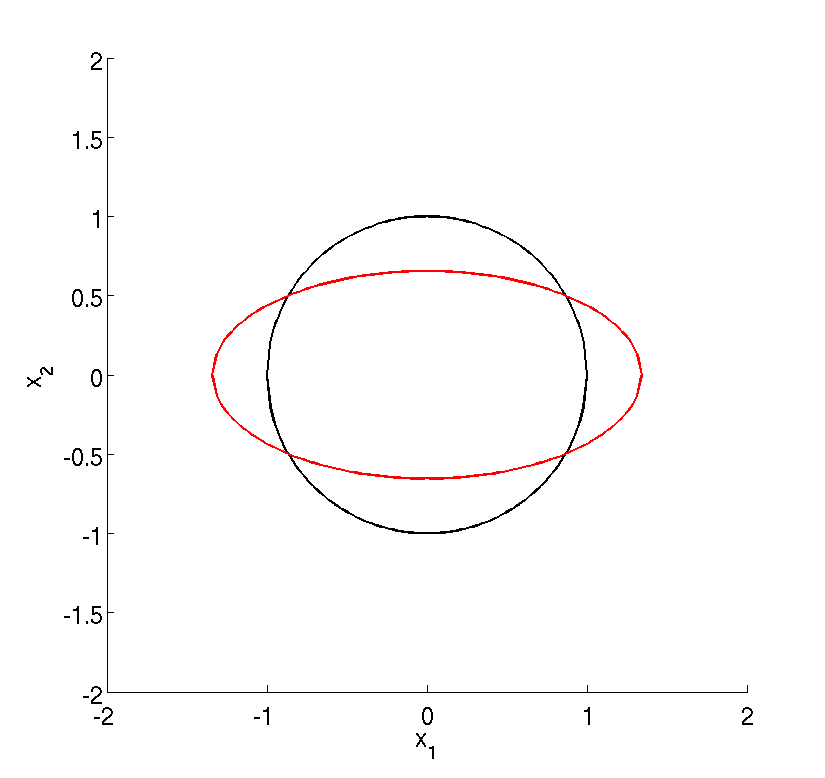
\includegraphics[width=\textwidth]{figures/P1}
    \end{column}
    %
  \end{columns}

\end{frame}

\subsection{Contraction mapping}

\begin{frame}
  \frametitle{Contraction mapping}

  Again find root $\bfm{s}$ by constructing sequence $\{ \bfm{x}_n \}$
  using map ${\mathbf g}: {\mathbb R}^n \rightarrow {\mathbb R}^n$:
  \begin{equation*}
     \bfm{x}_{n+1} = \bfm{g} (\bfm{x}_n)
  \end{equation*} \pause

  In analogy with scalar case define interval $I$ as
  \begin{equation*}
    I = \{ \bfm{x} \in {\mathbb R}^n \,\, | \, a_j < x_j < b_j, \,\, j
    = 1, 2, \dots, n \}.
  \end{equation*} \pause

  Hence define contraction map as a Lipschitz continuous map
  $\bfm{g}(\bfm{x})$ such that $\bfm{g}(I) \subseteq I$ and with
  Lipschitz constant $L < 1$:
  \begin{equation*}
    \| \bfm{g}(\bfm{x}) - \bfm{g}(\bfm{y}) \| \leq L \| \bfm{x} -
    \bfm{y} \| \quad \forall \bfm{x}, \bfm{y} \in I.
  \end{equation*}

\end{frame}


\begin{frame}
  \frametitle{Contraction mapping theorems}

  {\bf Theorem}: If $\bfm{g}$ is continuous in $I$ and $\bfm{g}(I)
  \subseteq I$ then $\bfm{g}$ has at least one fixed point in $I$.
  \pause

  \vspace{1ex}

  {\bf Contraction mapping theorem in $\mathbf{R}^n$}: If
  $\bfm{g}(\bfm{x})$ is a contraction mapping in $I$ then there exists
  one and only one fixed point in $I$. \pause

  \vspace{1ex}

  {\bf Theorem}: If $\bfm{g}(\bfm{x})$ is a contraction mapping in $I$
  then for arbitrary $\bfm{x}_0 \in I$ then the sequence $\{ \bfm{x}_n
  \}$ converges to the unique fixed point with error
  \begin{equation*}
    \| \bfm{e}_n \|_{\infty} \leq \frac{L^n}{1 - L} \| \bfm{x}_1 -
    \bfm{x}_0 \|_{\infty}.
  \end{equation*} \pause

  {\bf Theorem}: If $\bfm{g}(\bfm{x})$ is a differentiable contraction
  map in $I$, i.e.\
  \begin{equation*}
    \left| \frac{\partial g_i}{\partial x_j} \right| \leq \frac{L}{n},
  \end{equation*}
  then there exists one and only one fixed point in $I$.

\end{frame}


\begin{frame}
  \frametitle{Example}

  Look at map
  \begin{equation*}
    \bfm{g}(\bfm{x}) = \left\{
      \begin{aligned}
        g_1 (x_1, x_2, x_3) & = \tfrac{1}{3} \cos( x_2 x_3 ) +
        \tfrac{1}{6} \\
        g_2 (x_1, x_2, x_3) & = \tfrac{1}{9} \sqrt{x_1^2 + \sin{x_3} +
        1.06} - 0.1 \\
        g_3 (x_1, x_2, x_3) & = -\tfrac{1}{20} \exp(-x_1 x_2) - (10
        \pi - 3) / 60
      \end{aligned}
    \right. .
  \end{equation*} \pause

  By computing the Jacobian of the map
  \begin{equation*}
    J(\bfm{x}) =
    \begin{pmatrix}
      0 & -\tfrac{1}{3} \sin(x_2 x_3) x_3 &  -\tfrac{1}{3} \sin(x_2
      x_3) x_2 \\
      \tfrac{1}{9} \frac{x_1}{\sqrt{x_1^2 + \sin(x_3) + 1.06}} & 0 &
      \tfrac{1}{18} \frac{\cos(x_3)}{\sqrt{x_1^2 + \sin(x_3) + 1.06}}
      \\
      \tfrac{1}{20} x_2 \exp(-x_1 x_2) & \tfrac{1}{20} x_1 \exp(-x_1
      x_2) & 0
    \end{pmatrix}
  \end{equation*}
  see that all elements of $J$ are less than $1/3$ in magnitude in
  $I = [-1,1]^3$. Hence there is a unique fixed point in $I$.

\end{frame}

\begin{frame}
  \frametitle{Example: 2}

  Iterate starting from $\bfm{x} = (0.2, 0.3, 0.4)$: appears to converge to a fixed point
  \begin{center}
    \begin{tabular}{c|c c c}
      $n$ & $x_1$ & $x_2$ & $x_3$ \\ \hline
      0 & 0.2 & 0.3 & 0.4 \\
      1 & 0.4976029  &  0.0356019 &  -0.5206870 \\
      2 & 0.4999427  &  0.0000082 &  -0.5227208 \\
      3 & 0.5000000  &  0.0000434 &  -0.5235986 \\
      4 & 0.5000000  &  0.0000000 &  -0.5235977 \\
      5 & 0.5000000  &  0.0000001 &  -0.5235988
    \end{tabular}
  \end{center}

\end{frame}

\begin{frame}
  \frametitle{Example: 3}

  \begin{center}
    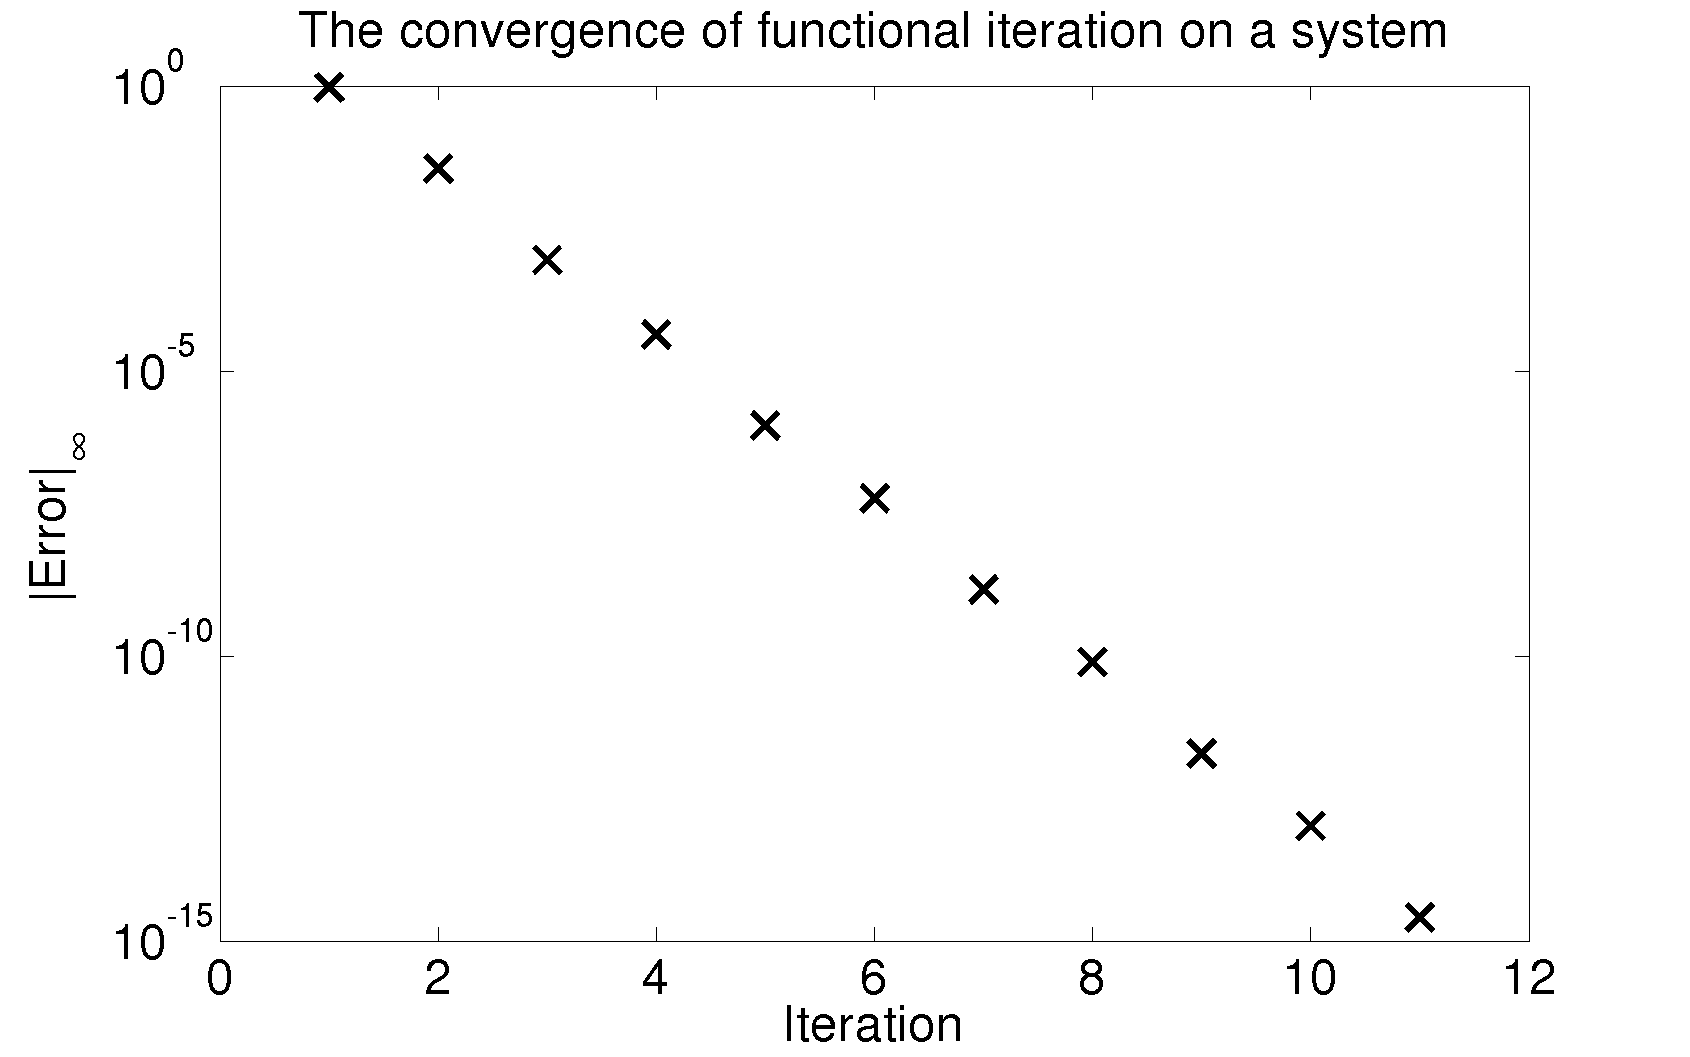
\includegraphics[height=0.7\textheight]{figures/NonlinearSystemExample1}
  \end{center}
  Convergence is linear, as usual.  Geometric picture not straightforward.

\end{frame}

\begin{frame}
  \frametitle{Geometric picture}

  \begin{center}
    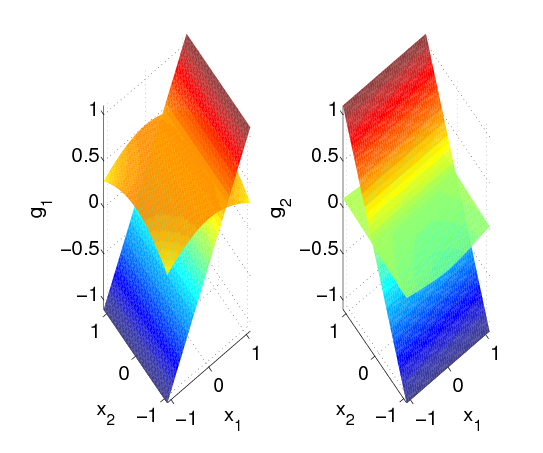
\includegraphics[height=0.7\textheight]{figures/NonlinearSystemGeom1}
  \end{center}
  Trying to find unique point giving the intersection of
  \emph{each} map with the appropriate axis plane; we move along each
  in turn.

\end{frame}


\begin{frame}
  \frametitle{(Non)linear systems analogies}

  Consider e.g.\ Jacobi for $A \bfm{x} = \bfm{b}$: constructs sequence $\{ \bfm{x}_n\}$ with correct answer in the limit. Analogous to iterative methods here. \pause Inspires:
  %
  \begin{enumerate}
  \item ``Gauss-Seidel'': use guess as soon as possible. I.e.,
    \begin{align*}
      &&(x_1)_{n+1} & = g_1\left((x_1)_n, (x_2)_n\right) \\
      \text{then }&& (x_2)_{n+1} &= g_2\left((x_1)_{n+1}, (x_2)_n\right).
    \end{align*}
  \item ``Relaxation'': $\hat{\bfm{x}}_{n+1} = \bfm{g}(\bfm{x}_n)$, but
    \emph{actual} next iterate uses  ``correction'' as
    \begin{equation*}
      \bfm{x}_{n+1} = \bx_n + \omega (\hat{\bx}_{n+1} - \bx_n).
    \end{equation*}
    Typically take $\omega < 1$ to promote convergence
    (\emph{under} relaxation); can be impractical (slow).
  \end{enumerate}

  % \begin{overlayarea}{\textwidth}{0.9\textheight}
  %   \only<1|handout:1>
  %   {

  %     At each stage we are using an iterative method to find a new
  %     member of a sequence, looking for a limit that
  %     will give us the correct answer. This clearly has an analogy
  %     with iterative methods for solving linear systems: the key
  %     difference is that here the mapping is given by $\bfm{g}$, a
  %     nonlinear function.
  %   }
  %   \only<2|handout:2>
  %   {
  %     We can still make use of the analogy to linear systems by
  %     considering two methods inspired by them:
  %     \begin{enumerate}
  %     \item A ``Gauss-Seidel'' version where the value of the guess is
  %       used as soon as possible. I.e., if $\{(x_1)_n, (x_2)_n\}$ are used
  %       to compute
  %       \begin{align*}
  %         &&(x_1)_{n+1} & = g_1\left((x_1)_n, (x_2)_n\right) \\
  %         \text{then }&& (x_2)_{n+1} &= g_2\left((x_1)_{n+1}, (x_2)_n\right).
  %       \end{align*}
  %     \item A ``relaxation'' type method where the map is used to guess
  %       the next iterate, $\hat{\bfm{x}}_{n+1} = \bfm{g}(\bfm{x}_n)$, but
  %       the \emph{actual} next iterate is instead given by computing the
  %       ``correction'' as
  %       \begin{equation*}
  %         \bfm{x}_{n+1} = \bx_n + \omega (\hat{\bx}_{n+1} - \bx_n).
  %       \end{equation*}
  %       Typically we take $\omega < 1$ to promote convergence
  %       (\emph{under} relaxation); this can lead to this method being
  %       impractical.
  %     \end{enumerate}
  %   }
  % \end{overlayarea}

\end{frame}

\subsection{Newton's method in two dimensions}

\begin{frame}
  \frametitle{Newton's method -- graphical approach}

  ``Best'' method in scalar case: Newton iteration.

  \vspace{1ex}

  \begin{columns}[T]
    \begin{column}{0.5\textwidth}
      Scalar geometric picture: follow tangent from curve to axis. \pause

      Derive using Taylor expansion:
      \begin{align*}
        z &= f(x_n) + (x - x_n) f'(x_n) \\
        z & = 0 \quad \implies \quad x_{n+1} = x_n - \frac{f(x_n)}{f'(x_n)}.
      \end{align*} \pause

      System geometric picture: follow tangent \emph{planes}. \pause Apply to each component (map). \pause Find mutual intersections.
    \end{column}
    \begin{column}{0.5\textwidth}
      \includegraphics<1-2|handout:0>[height=0.6\textheight]{figures/Newton}
      \includegraphics<3|handout:0>[width=\textwidth]{figures/krd_plane2}
      \includegraphics<4->[width=\textwidth]{figures/krd_plane3}\\
      \includegraphics<5>[width=\textwidth]{figures/krd_plane4}
    \end{column}
  \end{columns}

\end{frame}

% \begin{frame}
%   \frametitle{Newton's method -- Graphical interpretation}

%   In solving a single nonlinear equation, Newton's method gave the
%   fastest convergence of the methods introduced. Quadratic convergence
%   was obtained if we started sufficiently close to the root. We would
%   obviously like a similar algorithm for a system. \pause

%   \begin{overlayarea}{\textwidth}{0.7\textheight}
%     \begin{columns}[T]
%       \begin{column}{0.5\textwidth}
%         \only<2->
%         {
%           \vspace{5ex}
%           One way of thinking about Newton's method is geometrically:
%           the next iterate is found by drawing the line tangent to the
%           curve at this iterate and following down to the axis.
%         }
%       \end{column}
%       \begin{column}{0.5\textwidth}
%         \begin{center}
%           \includegraphics<2->[height=0.6\textheight]{Newton}
%         \end{center}
%       \end{column}
%     \end{columns}
%   \end{overlayarea}
% \end{frame}
% \begin{frame}
%   \frametitle{Newton's method -- Graphical interpretation}
%   The graphical interpretation gives an intuitive view of how Newton's method generalises to two dimensions. \pause
%   Mathematically this is derived by considering the linearisation of the functions about the point $x_n,y_n$. \pause
%   In 1D this can be done through a Taylor expansion
%   %
%   \begin{equation*}
%     z = f(x_n)+(x-x_n)f'(x_n).
%   \end{equation*}
%   %
%   \pause
%   The next iterate is given by the point where the line intersects the axis $z=0$,
%   %
%   \begin{equation*}
%     x_{n+1} = x_n - \frac{f(x_n)}{f'(x_n)}.
%   \end{equation*}
%   %
% \end{frame}

% \begin{frame}
%   \frametitle{Newton's method -- Graphical interpretation}

%   We consider the extension to two dimensions.  Suppose we want to
%   solve $f_1(x,y)=0$ and $f_2(x,y)=0$ using a Newton iterative scheme.
%   \pause
%   \begin{columns}[T]
%       \begin{column}{0.4\textwidth}
% 	\vspace{7mm}
% 	In 1D we considered the line tangent to the curve at the point $x_n$. \pause
% 	In 2D we consider the plane tangent to the curve at the point
% 	$x_n,y_n$ to derive the new point $x_{n+1},y_{n+1}$.
%       \end{column}
%       \begin{column}{0.55\textwidth}
% 	\begin{overlayarea}{\textwidth}{0.5\textheight}
% 	  \begin{center}
%             \includegraphics<1>[width = \textwidth]{krd_plane1}
%             \includegraphics<2->[width = \textwidth]{krd_plane2}
%           \end{center}
% 	\end{overlayarea}
%       \end{column}
%     \end{columns}
%   \pause
%   The next iterate is given by the point at which the two planes intersect the coordinate axis.
% \end{frame}

% \begin{frame}
%   \frametitle{Newton's method -- Graphical interpretation}
%    \begin{columns}[T]
%       \begin{column}{0.5\textwidth}
% 	  \begin{center}
%             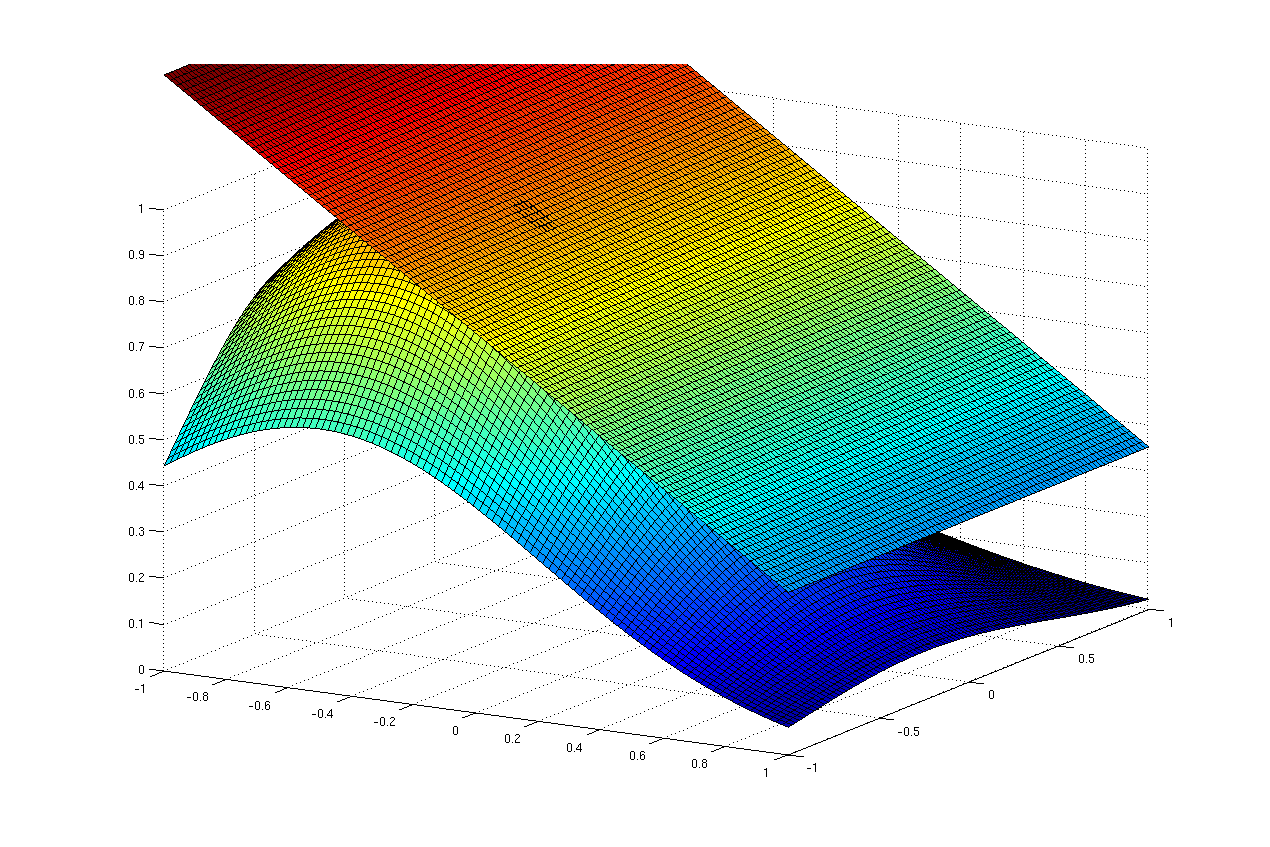
\includegraphics[width = 0.8\textwidth]{krd_plane2}
%           \end{center}
%       \end{column}
%       \begin{column}{0.5\textwidth}
% 	  \begin{center}
%             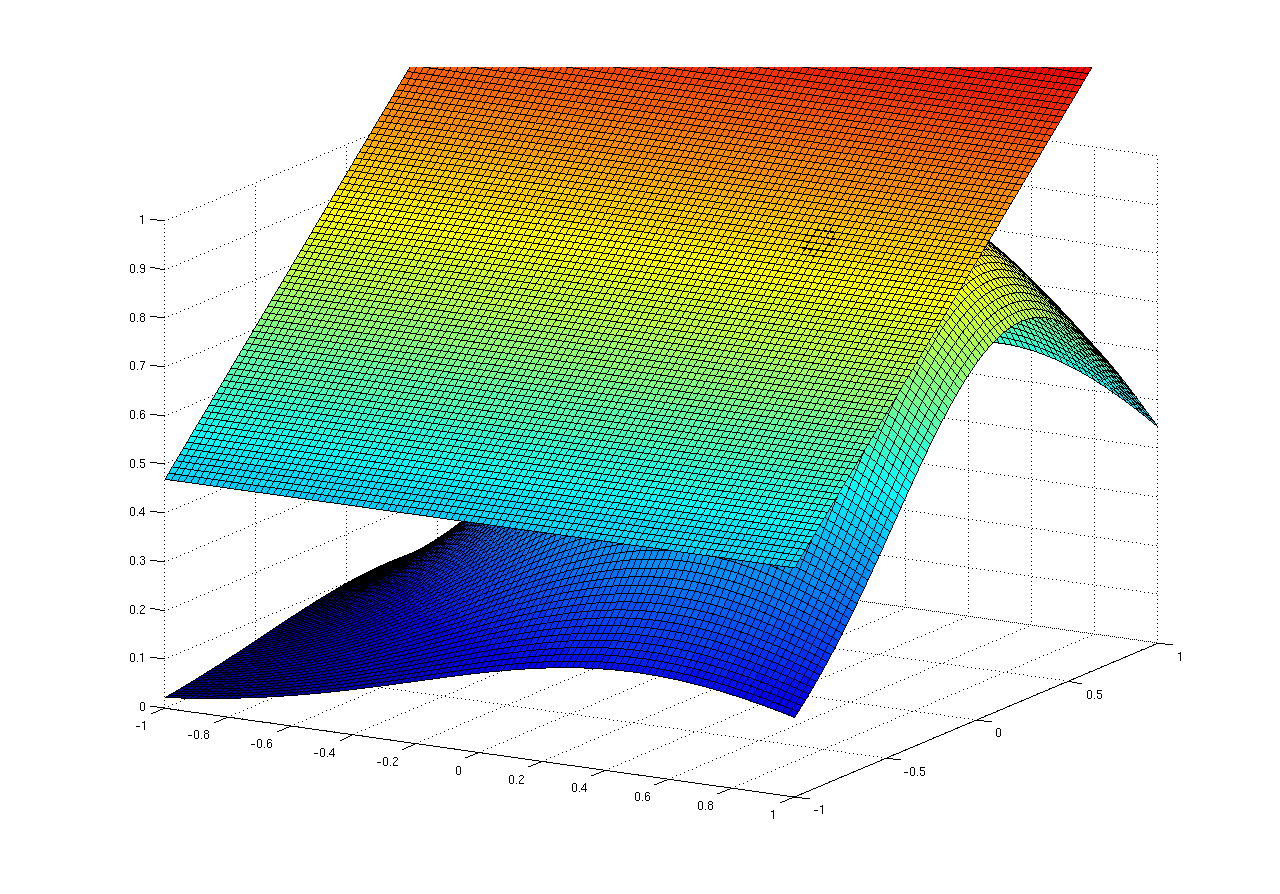
\includegraphics[width = 0.8\textwidth]{krd_plane3}
%           \end{center}
%       \end{column}
%     \end{columns}
% %
%     \begin{center}
%       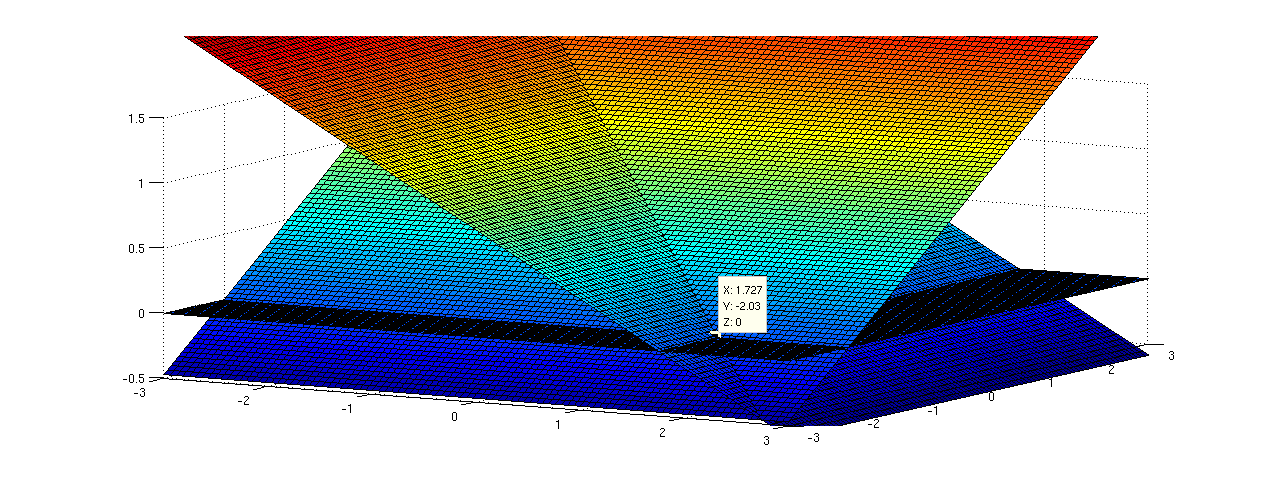
\includegraphics[width = 0.9\textwidth]{krd_plane4}
%     \end{center}
% \end{frame}

\begin{frame}
  \frametitle{Newton's method from Taylor series}

  The planes tangent to the surface are given by the Taylor expansion
  %
  \begin{align*}
    z_1 = & f_1 (x_n,y_n) + (x - x_n) \frac{\partial
      f_1}{\partial x}+ (y - y_n) \frac{\partial
      f_1}{\partial y}, \\
    z_2 = &f_2 (x_n,y_n) + (x - x_n) \frac{\partial
      f_2}{\partial x}+ (y - y_n) \frac{\partial
      f_2}{\partial y}.
  \end{align*} \pause
  Set $z_1=0$, $z_2=0$ to find next iterate.
  %
  \begin{align*}
    \begin{pmatrix}
      \pda{f_1}{x} & \pda{f_1}{y} \\ \pda{f_2}{x} & \pda{f_2}{y}
    \end{pmatrix}
    \begin{pmatrix}
      x_{n+1} - x_{n} \\ y_{n+1} - y_{n}
    \end{pmatrix}
    =
    \begin{pmatrix}
      -f_1 (x_n,y_n) \\ -f_2 (x_n,y_n)
    \end{pmatrix}.
  \end{align*}\pause
  %
  This can be written as a matrix equation
  \begin{equation*}
    J (\bx_n) \cdot ( \bx_{n+1} - \bx_n ) = -( \bfm{f}(\bx_n))
  \end{equation*}
  where $J$ is the \emph{Jacobian} matrix. \pause
  Therefore the iteration scheme is
  \begin{equation*}
    \bx_{n+1} = \bx_n - J^{-1} \bfm{f}(\bx_n).
  \end{equation*}

\end{frame}

\begin{frame}
  \frametitle{Newton's method algorithm}

  Final algorithm. Given guess $\bx_0 \implies \bx_n$. At step $n+1$:
  %
  \begin{enumerate}
  \item Compute $\bfm{f}(\bx_n)$.
  \item Compute Jacobian $J (\bx_n)$.
  \item Solve for ``correction'' $\bfm{c}$ from $J (\bx_n) \bfm{c} = -\bfm{f}(\bx_n)$.
  \item Compute $\bx_{n+1} = \bx_n + \bfm{c}$.
  \end{enumerate} \pause
  %

  Never invert Jacobian explicitly.

  \vspace{1ex}

  Newton's method is computationally expensive: generalization of secant method exists.

\end{frame}

\begin{frame}
  \frametitle{Simple example revisited}

  \begin{columns}
    %
    \begin{column}{0.5\textwidth}
      %
      Consider the system
      %
      \begin{align*}
        x_1^2 + x_2^2 - 1 & = 0 \\
        5 x_1^2 + 21 x_2^2 - 9 & = 0.
      \end{align*}
      %
      Have $\bx = (x_1, x_2)^T$, ${\bf f} = (f_1,
      f_2)^T$
      %
      \begin{align*}
        f_1(x_1, x_2) & = x_1^2 + x_2^2 - 1, \\
        f_2(x_1, x_2) & = 5 x_1^2 + 21 x_2^2 - 9.
      \end{align*}
      %
      \emph{Four} solutions ${\bf \xi} = (\pm \sqrt{3} /
      2, \pm 1 / 2)^T$. Match the four intersections of the
      two curves. \pause

      \vspace{1ex}

      Newton's method from $(1, 1)$ works.
      %
    \end{column}
    %
    \begin{column}{0.5\textwidth}
      \includegraphics<1|handout:0>[width=\textwidth]{figures/P1}
      \includegraphics<2>[width=\textwidth]{figures/NewtonExample}
    \end{column}
    %
  \end{columns}

\end{frame}

\section{Summary}

\subsection{Summary}

\begin{frame}
  \frametitle{Summary}

  \begin{itemize}
  \item The theory of contraction mapping essentially carries over to
    systems by replacing scalars with vectors and absolute values with
    norms.
  \item Analogies with solving systems of \emph{linear} equations
    leads to ``Gauss-Seidel'' and ``relaxation'' methods.
  \item Newton's method generalizes by considering tangent
    \emph{(hyper)planes}, which leads to a method based on the
    Jacobian matrix.
    \end{itemize}

\end{frame}

\end{document}





%%% Local Variables:
%%% mode: latex
%%% TeX-master: t
%%% End:
